\documentclass[11pt,twocolumn]{article}
\usepackage[letterpaper,margin=0.65in]{geometry}
\usepackage{amsmath,graphicx,booktabs}
\usepackage{times}
\setlength{\columnsep}{0.24in}
\setlength{\textfloatsep}{7pt plus 2pt minus 2pt}
\setlength{\intextsep}{7pt plus 2pt minus 2pt}
\setlength{\abovecaptionskip}{4pt}
\title{Computing Pi with OpenMP:\\Synchronization, Scaling, and Accuracy}
\author{CS 431/531 -- Homework 01}
\date{}
\begin{document}
\maketitle

\section{Methods}
Lecture 5 (slides 43--46) introduces rectangle integration of a semicircle.
By symmetry, $\pi=4\int_0^1\sqrt{1-x^2}\,dx$. The implementation uses
midpoint rectangles on this quarter-circle:
\[
 \widehat{\pi}_N=\frac{4}{N}\sum_{i=0}^{N-1}
 \sqrt{1-\left(\frac{i+1/2}{N}\right)^2}.
\]
The serial implementation is the correctness baseline. Two OpenMP
\texttt{parallel for} versions update a shared sum once per slice,
using either \texttt{critical} or \texttt{atomic}. An additional
\texttt{reduction(+:sum)} version accumulates private sums before combining
them, separating synchronization costs from useful work.

For Monte Carlo, $N$ points are generated in $[0,1)^2$. If $H$ lie inside
the quarter-circle, the estimate is $4H/N$. A SplitMix64-based counter
generator assigns each sample its own two random coordinates; there is no
shared random-number state. An integer OpenMP reduction counts hits.
The same seed gives identical points and estimates at every thread count.
Numerical tests check all integration methods against an independent
quadrature calculation and the sampling method against a Python RNG oracle.

\section{Experimental setup}
All reported measurements came from Talapas job \texttt{48008499} on
\texttt{n0135}, on October 21, 2026. The node has two AMD EPYC 7713
64-core processors; the job allocated 32 physical cores and 4\,GiB RAM.
GCC 8.5.0 compiled the program with \texttt{-O3 -fopenmp}, without
fast-math. OpenMP used static scheduling, core places, spread binding,
passive waiting, and disabled dynamic teams.

Thread counts were 1, 2, 4, 8, 16, and 32. Serial, reduction, and Monte
Carlo used $N=10^4,\ldots,10^8$; the critical/atomic study stopped at
$10^6$ to bound contention costs. Each of the 101 configurations had
20 timed runs after an untimed warm-up: 2,020 measurements in total.
Configurations were shuffled in a fixed random order; runs within each
configuration were consecutive. Timings use \texttt{omp\_get\_wtime},
include fork/join and barriers, and exclude output. Means and sample
standard deviations summarize timing. Monte Carlo uses 20 seeds,
$431531,\ldots,431550$, reused across thread counts for paired comparisons.

\begin{figure}[t]
\centering
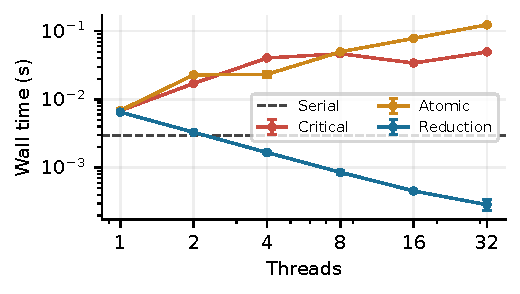
\includegraphics[width=\columnwidth]{figures/synchronization.pdf}
\caption{Integration at $N=10^6$: mean wall time and $\pm1$ sample
standard deviation over 20 runs. Both axes use logarithmic scales.}
\label{fig:sync}
\end{figure}

\section{Performance}
Figure~\ref{fig:sync} shows that synchronization per slice overwhelms
the work of evaluating a square root. At 32 threads and $10^6$ slices,
critical took $49.45\pm0.58$\,ms, atomic $123.34\pm0.58$\,ms, and reduction
$0.287\pm0.050$\,ms. The serial baseline took $2.926\pm0.004$\,ms.
Thus critical and atomic were respectively 16.9 and 42.2 times slower
than serial, while reduction was about 10.2 times faster at this size.
Atomic was not inherently faster than a critical section on this system.
Both contend on one shared sum; compiler/runtime details and contention
matter more than the shorter source directive. These timings alone do
not identify the precise hardware cause of their ordering.

\begin{figure}[t]
\centering
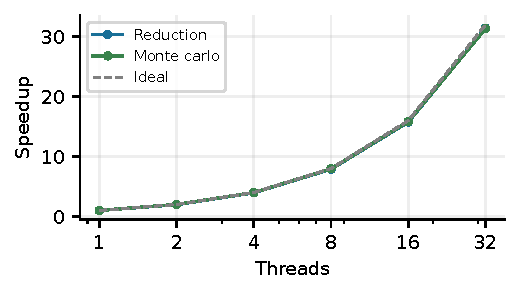
\includegraphics[width=\columnwidth]{figures/scaling.pdf}
\caption{Strong scaling at $N=10^8$. Each speedup uses that method's
own one-thread mean; the dashed line is ideal scaling.}
\label{fig:scale}
\end{figure}

For the larger workload in Figure~\ref{fig:scale}, reduction improved
from 650.25\,ms at one thread to 20.69\,ms at 32 threads, a $31.42\times$
speedup. Monte Carlo improved from 336.97\,ms to 10.74\,ms, or
$31.37\times$. These are within-method speedups: the separate serial
integration was faster than one-thread OpenMP reduction (292.18\,ms).
Relative to that serial baseline, 32-thread reduction accelerated the
integration by $14.12\times$, not $31.42\times$. Small workloads amortize
thread startup less effectively; the corresponding reduction speedup
against its own baseline at $N=10^6$ was only $22.70\times$.

\section{Accuracy and limitations}
Figure~\ref{fig:accuracy} uses serial midpoint absolute error and Monte
Carlo root-mean-square error (RMSE) across the 20 seeds. Increasing the
thread count changes integration's floating-point summation order but
does not improve its discretization, and it does not increase the number
of Monte Carlo samples. The sampled estimates were exactly identical
across thread counts at fixed $N$ and seed; those repeated estimates
were therefore not pooled as additional independent observations.

\begin{figure}[t]
\centering
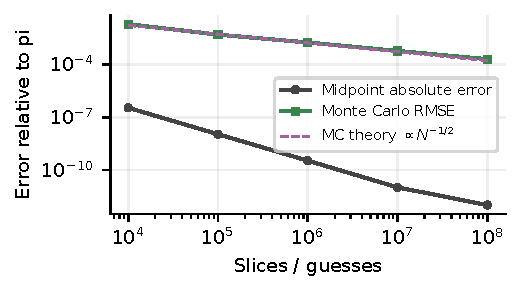
\includegraphics[width=\columnwidth]{figures/accuracy.pdf}
\caption{Accuracy versus slices/guesses. Monte Carlo uses 20 seeds;
the theory line is $\sqrt{(4\pi-\pi^2)/N}$. Integration is deterministic
apart from rounding. Errors are relative to double-precision $\pi$.}
\label{fig:accuracy}
\end{figure}

Midpoint error fell from $3.44\times10^{-7}$ at $10^4$ slices to
$1.05\times10^{-12}$ at $10^8$. The quarter-circle integrand has a
singular derivative at $x=1$; its observed pre-roundoff convergence is
approximately $N^{-3/2}$, rather than the usual smooth-integrand
midpoint $N^{-2}$ expectation. At the largest size, rounding and
summation order affect the remaining error.
Monte Carlo RMSE fell from $1.90\times10^{-2}$ to $1.97\times10^{-4}$,
consistent with the slower $N^{-1/2}$ trend. Its uncertainty does not
decrease monotonically for individual seeds, and 20 seeds give a noisy
estimate of RMSE. For this one-dimensional circle-area problem,
quadrature achieves much higher accuracy per evaluation.

These results describe one allocation on one shared node, with
consecutive repetitions per configuration; they are not cross-node or
cross-day confidence claims. Error bars are standard deviations, not
confidence intervals. Raw CSV, job logs, and the plotting script
accompany this report so the figures can be reproduced.
The main lesson is to reduce private partial results rather than
serialize every update, and to distinguish parallel speedup from
statistical accuracy.
\end{document}
